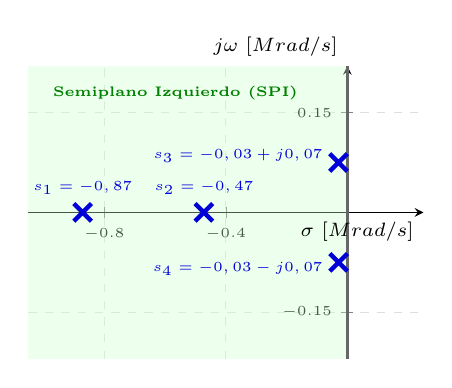
\begin{tikzpicture}
  \begin{axis}[
    width=6.6cm, height=5.3cm,
    axis lines=middle,
    xlabel={$\sigma$ [$\text{Mrad/s}$]},
    ylabel={$j\omega$ [$\text{Mrad/s}$]},
    xlabel style={at={(ticklabel* cs:1)}, anchor=north east, font=\scriptsize},
    ylabel style={at={(ticklabel* cs:1)}, anchor=south east, font=\scriptsize},
    xmin=-1.05, xmax=0.25, ymin=-0.22, ymax=0.22,
    xtick={-0.8, -0.4, 0},
    ytick={-0.15, 0.15},
    grid=both, grid style={gray!25, dashed},
    tick label style={font=\tiny},
  ]
    % Zona estable LHP sombreada
    \fill[green!20, opacity=0.35] (axis cs:-1.05,-0.22) rectangle (axis cs:0,0.22);

    % Eje jw (frontera)
    \draw[line width=1.0pt, black!60] (axis cs:0,-0.22) -- (axis cs:0,0.22);

    % Polos reales LHP
    \addplot[only marks, mark=x, mark size=4.5pt, line width=1.6pt, blue!85!black]
      coordinates {(-0.871, 0) (-0.472, 0)};
    \node[above=3pt, blue!85!black, font=\tiny\bfseries, anchor=south] at (axis cs:-0.871, 0) {$s_1 = -0,87$};
    \node[above=3pt, blue!85!black, font=\tiny\bfseries, anchor=south] at (axis cs:-0.472, 0) {$s_2 = -0,47$};

    % Polos complejos LHP (estables)
    \addplot[only marks, mark=x, mark size=4.5pt, line width=1.6pt, blue!85!black]
      coordinates {(-0.029, 0.075) (-0.029, -0.075)};
    \node[blue!85!black, font=\tiny\bfseries, anchor=east] at (axis cs:-0.05, 0.085) {$s_{3} = -0,03 + j0,07$};
    \node[blue!85!black, font=\tiny\bfseries, anchor=east] at (axis cs:-0.05, -0.085) {$s_{4} = -0,03 - j0,07$};

    \node[green!50!black, font=\tiny\bfseries, anchor=west] at (axis cs:-1.0, 0.18) {Semiplano Izquierdo (SPI)};
  \end{axis}
\end{tikzpicture}
